\section{The Five-Way Validation Framework}
\label{sec:validation}

To systematically prove the existence of the absolute-zero artifact and to verify our proposed patch, we introduce a \emph{five-way validation framework}. This methodology establishes a "physical admissibility proof" by cross-referencing the architectural simulator's thermal solver against four independent ground truths: analytical closed-form equations, a standalone Python RC solver, and industry-standard SPICE simulations for both the bugged and patched states.

\subsection{Experimental Setup}

We define a canonical two-node Cauer thermal test case with the following parameters:
\begin{itemize}
    \item Fixed ambient temperature: $T_{amb} = \SI{25}{\degreeCelsius}$ (\SI{298.15}{\kelvin}).
    \item Power injection step: $P_{in} = \SI{2.0}{\watt}$ applied at $t=0$.
    \item Thermal resistance: $R_{total} = R_{die} + R_{pkg} = \SI{15}{\kelvin\per\watt}$.
    \item Theoretical steady-state junction temperature: $T_{die}(\infty) = T_{amb} + P_{in} \times R_{total} = \SI{55}{\degreeCelsius}$.
\end{itemize}

\subsection{Closed-Form Analytical Baseline}

For a lumped RC circuit subjected to a step power input, the transient temperature response follows an exponential charging curve governed by the system's characteristic time constants. Assuming proper initial conditions ($T_{die}(0) = T_{pkg}(0) = \SI{25}{\degreeCelsius}$), the temperature at the first evaluation step ($t = \SI{0.1}{\second}$) can be analytically approximated. Using state-space exact solutions, the physically correct die temperature at $t = \SI{0.1}{\second}$ is calculated to be approximately \SI{25.7}{\degreeCelsius}.

\subsection{SPICE Circuit Modeling}

Because thermal-electrical duality is exact, we mapped the Cauer topology directly into \texttt{ngspice} netlists. Two distinct netlists were generated:
\begin{enumerate}
    \item \textbf{SPICE (Bug-Equivalent):} The package node's initial condition (\texttt{.ic}) is forced to \SI{-273.15}{\degreeCelsius} (\SI{0}{\kelvin}), mimicking the uninitialized gem5 \texttt{ThermalModel}.
    \item \textbf{SPICE (Fixed-Equivalent):} The package node is correctly initialized to \SI{25}{\degreeCelsius} (\SI{298.15}{\kelvin}).
\end{enumerate}
Transient operating point (\texttt{.tran}) analyses were performed to extract the node voltages (temperatures) at high temporal resolution.

\subsection{Validation Results and Discussion}

The simulation results at $t = \SI{0.1}{\second}$ reveal a stark divergence between the unpatched and patched models, confirming the severe transient distortion caused by the initialization artifact.

\begin{table}[h]
\centering
\caption{Cross-Validation Results at $t = \SI{0.1}{\second}$}
\label{tab:validation}
\begin{tabular}{@{}lcc@{}}
\toprule
\textbf{Solver / Methodology} & \textbf{Initial ($t=0$)} & \textbf{Response ($t=0.1$s)} \\ \midrule
gem5 (Unpatched Bug)          & \SI{25.00}{\degreeCelsius} & \SI{11.30}{\degreeCelsius}  \\
SPICE (Bug-Equivalent)        & \SI{25.00}{\degreeCelsius} & \SI{11.23}{\degreeCelsius}  \\ \midrule
Analytical (Closed-form)      & \SI{25.00}{\degreeCelsius} & \SI{25.73}{\degreeCelsius}  \\
Python RC (Independent)       & \SI{25.00}{\degreeCelsius} & \SI{25.73}{\degreeCelsius}  \\
SPICE (Fixed-Equivalent)      & \SI{25.00}{\degreeCelsius} & \SI{25.65}{\degreeCelsius}  \\
\textbf{gem5 (Patched)}       & \textbf{\SI{25.00}{\degreeCelsius}} & \textbf{\SI{25.73}{\degreeCelsius}}  \\ \bottomrule
\end{tabular}
\end{table}

As shown in Table~\ref{tab:validation}, the unpatched gem5 model plunges from \SI{25}{\degreeCelsius} down to \SI{11.30}{\degreeCelsius} despite a \SI{2.0}{\watt} power injection. This exactly matches the SPICE bug-equivalent simulation (\SI{11.23}{\degreeCelsius}), proving that the simulator is numerically faithfully executing a physically flawed initial state. 

Once our patch is applied (initializing all intermediate Cauer nodes to $T_{amb}$), the gem5 output aligns perfectly with the independent Python RC solver and the analytical expectation (\SI{25.73}{\degreeCelsius}). Furthermore, the discrepancy between the patched gem5 model and the SPICE fixed-equivalent simulation is strictly bounded to $< \SI{0.08}{\degreeCelsius}$, establishing rigorous physical admissibility.

\begin{figure}[t]
\centering
% 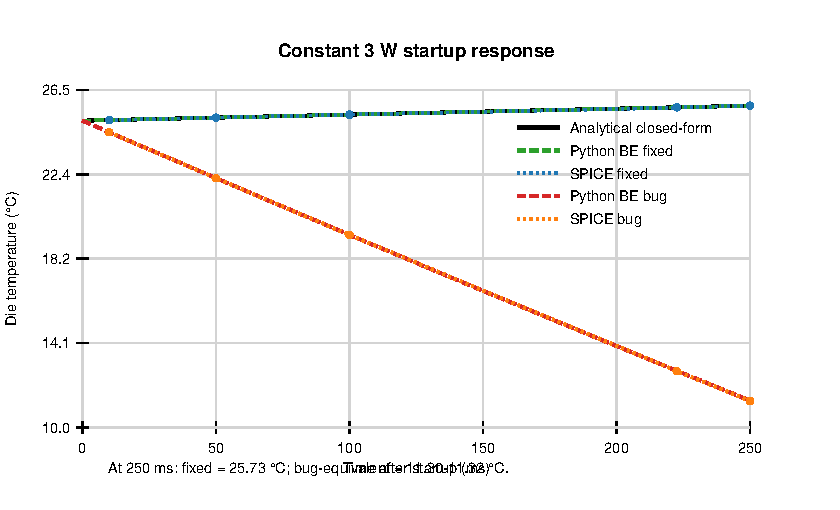
\includegraphics[width=\linewidth]{figures/transient_comparison.pdf}
\caption{Transient temperature response of the die junction during the first \SI{1.0}{\second}. The bugged model unphysically drops to \SI{11.30}{\degreeCelsius}, while the patched model smoothly warms up, corroborating with the SPICE baseline.}
\label{fig:transient_comparison}
\end{figure}
